\documentclass[conference]{IEEEtran}
\IEEEoverridecommandlockouts
% The preceding line is only needed to identify funding in the first footnote. If that is unneeded, please comment it out.
\usepackage{cite}
\usepackage{amsmath,amssymb,amsfonts}
\usepackage{algorithmic}
\usepackage{graphicx}
\usepackage{textcomp}
\usepackage{xcolor}
\def\BibTeX{{\rm B\kern-.05em{\sc i\kern-.025em b}\kern-.08em
    T\kern-.1667em\lower.7ex\hbox{E}\kern-.125emX}}
\begin{document}

\title{Modelling a reversible coupled wireless energy transfer system}

\author{\IEEEauthorblockN{1\textsuperscript{st} Edouard Bonnar}
\IEEEauthorblockA{
\textit{4th year Student} \\
\textit{Department of Computer and Electrical Engineering} \\
\textit{INSA-Toulouse}\\
Toulouse, France \\
bonnar-gaudr@insa-toulouse.fr}
\and
\IEEEauthorblockN{2\textsuperscript{nd} Flavien Carvalho}
\IEEEauthorblockA{
\textit{4th year Student} \\
\textit{Department of Computer and Electrical Engineering} \\
\textit{INSA-Toulouse}\\
Toulouse, France \\
fcarvalho@insa-toulouse.fr}
\and
\IEEEauthorblockN{3\textsuperscript{rd} Julie Champagne}
\IEEEauthorblockA{
\textit{4th year Student} \\
\textit{Department of Computer and Electrical Engineering} \\
\textit{INSA-Toulouse}\\
Toulouse, France \\
champagne@insa-toulouse.fr}
\and
\IEEEauthorblockN{4\textsuperscript{th} Denis Lespiaucq}
\IEEEauthorblockA{
\textit{4th year Student} \\
\textit{Department of Computer and Electrical Engineering} \\
\textit{INSA-Toulouse}\\
Toulouse, France \\
lespiaucq@insa-toulouse.fr}
\and
\IEEEauthorblockN{5\textsuperscript{th} Raphaël Marques}
\IEEEauthorblockA{
\textit{4th year Student} \\
\textit{Department of Computer and Electrical Engineering} \\
\textit{INSA-Toulouse}\\
Toulouse, France \\
rmarques@insa-toulouse.fr}
\and
\IEEEauthorblockN{6\textsuperscript{th} Caroline Nguyen}
\IEEEauthorblockA{
\textit{4th year Student} \\
\textit{Department of Computer and Electrical Engineering} \\
\textit{INSA-Toulouse}\\
Toulouse, France \\
c\_nguyen@insa-toulouse.fr}
\and
\IEEEauthorblockN{7\textsuperscript{th} Paul Pralus}
\IEEEauthorblockA{
\textit{4th year Student} \\
\textit{Department of Computer and Electrical Engineering} \\
\textit{INSA-Toulouse}\\
Toulouse, France \\
pralus@insa-toulouse.fr}
}

\maketitle

\begin{abstract}
Wireless power transfer, based on electromagnetic induction, is essential for short-range applications, particularly for mobile devices like electric vehicles and medical implants. However, coil misalignment can reduce transfer efficiency, requiring real-time measurement and optimization through a control algorithm. Additionally, for bidirectional systems such as vehicle-to-grid applications, the charger must support both battery charging and discharging. This research has two main objectives: to identify the parameters that will maximise the energy efficiency of the transfer, and then to calculate them and decide how to optimise the performance of wireless energy transfer in real time. It is built on previous work aimed at reducing the cost and weight of ferromagnetic materials while validating reversible power transfer. The methodology includes circuit modelling and simulation, followed by laboratory testing. It involves deriving a state-space model based on a simplified representation of the system using the first Fourier harmonic. The results enable real-time optimization of transfer efficiency using techniques such as mutual inductance measurement through the harmonics of the signal of the secondary coil applied to the primary coil with a radio communication link. The findings of this study had significant implications for improving contactless energy transfer systems, with potential applications in multiple fields. The next step will be to refine the models and conduct further tests to validate the proposed solutions. 
\end{abstract}

\section{Introduction}
The ongoing energy transition, driven by the increasing electrification of transportation and the rapid development of electric vehicles, presents new challenges in energy conversion. In particular, the growing demands for efficiency, safety, and bidirectional energy exchange in wireless charging systems have motivated the study andb optimization of high-performance converter topologies. 

In this context, the Dual Active Bridge (DAB) has emerged as a preferred architecture for high-power applications, such as fast charging of electric vehicles. Introduced in the 1990s, the DAB offers decisive advantages, including galvanic isolation via a high-frequency transformer, inherent capability for bidirectional energy transfer, and high efficiency operation through phase-shift modulation techniques. This topology also stands out for its robustness against geometric misalignments of coils in wireless power transfer systems, making it an ideal candidate for automated and intelligent charging infrastructures. 

Among the variety of existing DC/DC converters (Buck, Boost, Flyback, Resonant, etc.), the DAB is distinguished not only by its typical efficiency of over 95\%, but also by its control flexibility and compatibility with high-power charge/discharge requirements (up to several hundred kilowatts). Its ability to maintain optimal energy transfer even in cases of coil misalignment or load variations further enhances the appeal of this topology for advanced onboard or stationary systems. However, most research only applies to static misalignment and thus the parameters important for the optimization of the efficiency may vary over time.  

This article aims to explore in detail key elements to maximize efficiency of the DAB converter in imperfect conditions like coil misalignment through control of its bridges by a Pulse Width Modulation (PWM). 

\section{Related work}
Related Work DAB to condense in 1 page. If everything doesn’t fit we can do “Magouille \& compagnie” to put in elsewhere in the article

Related works -\> topology variants and technological choice?

\section{Methods}
\subsection{Electrical command}
As a way to control the DAB, it is possible to act on four parameters (including two parameters deduced from two others).  
\begin{figure}[htbp]
	\centerline{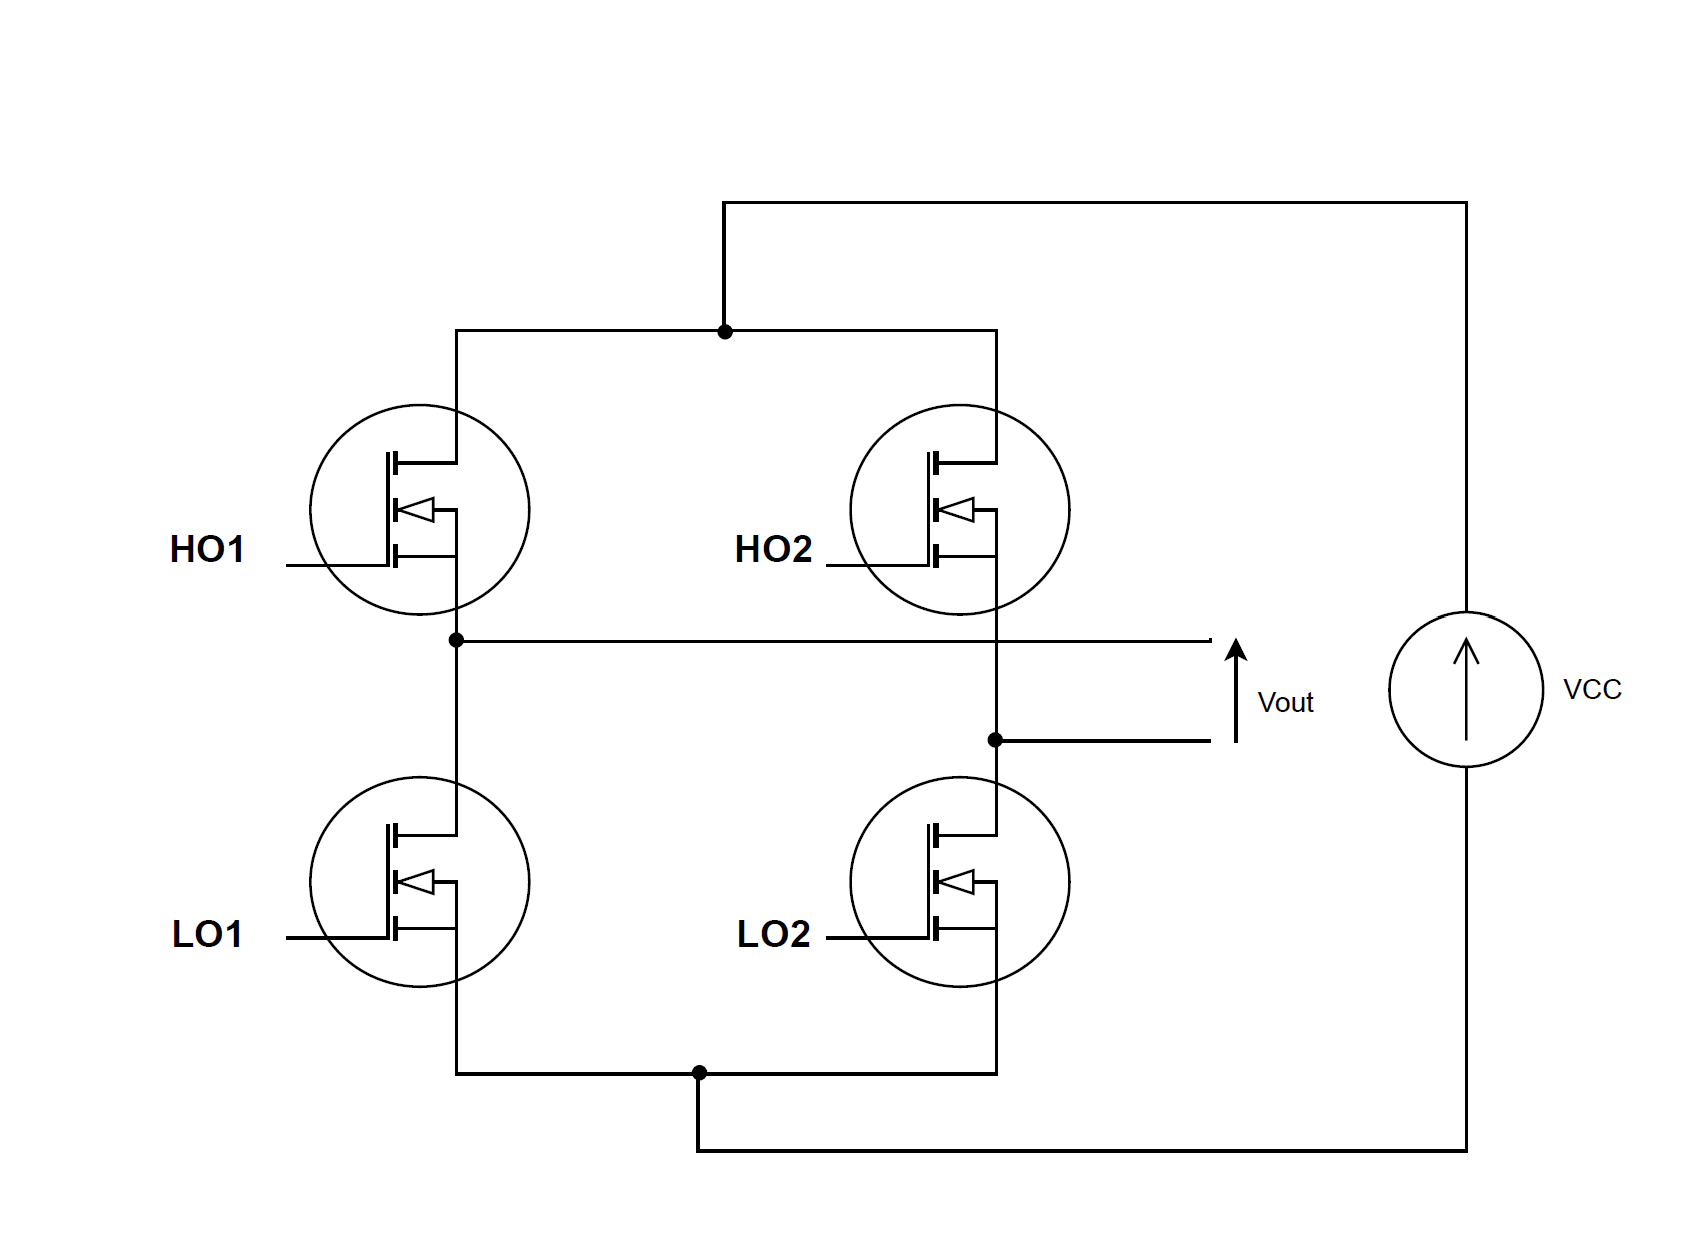
\includegraphics[width=\linewidth]{images/1.png}}
	\caption{H-Bridge electrical assembly}
	\label{fig}
\end{figure}

The duty cycle \( \alpha \) that must be included in the interval \([0\% ; 50\%[\) corresponds to the
percentage of the period where the pair of MOSFET transistors (on primary side) [Q1, Q4] are conducting and in addition, the pair [Q2, Q3] are off.

\begin{figure}[htbp]
	\centerline{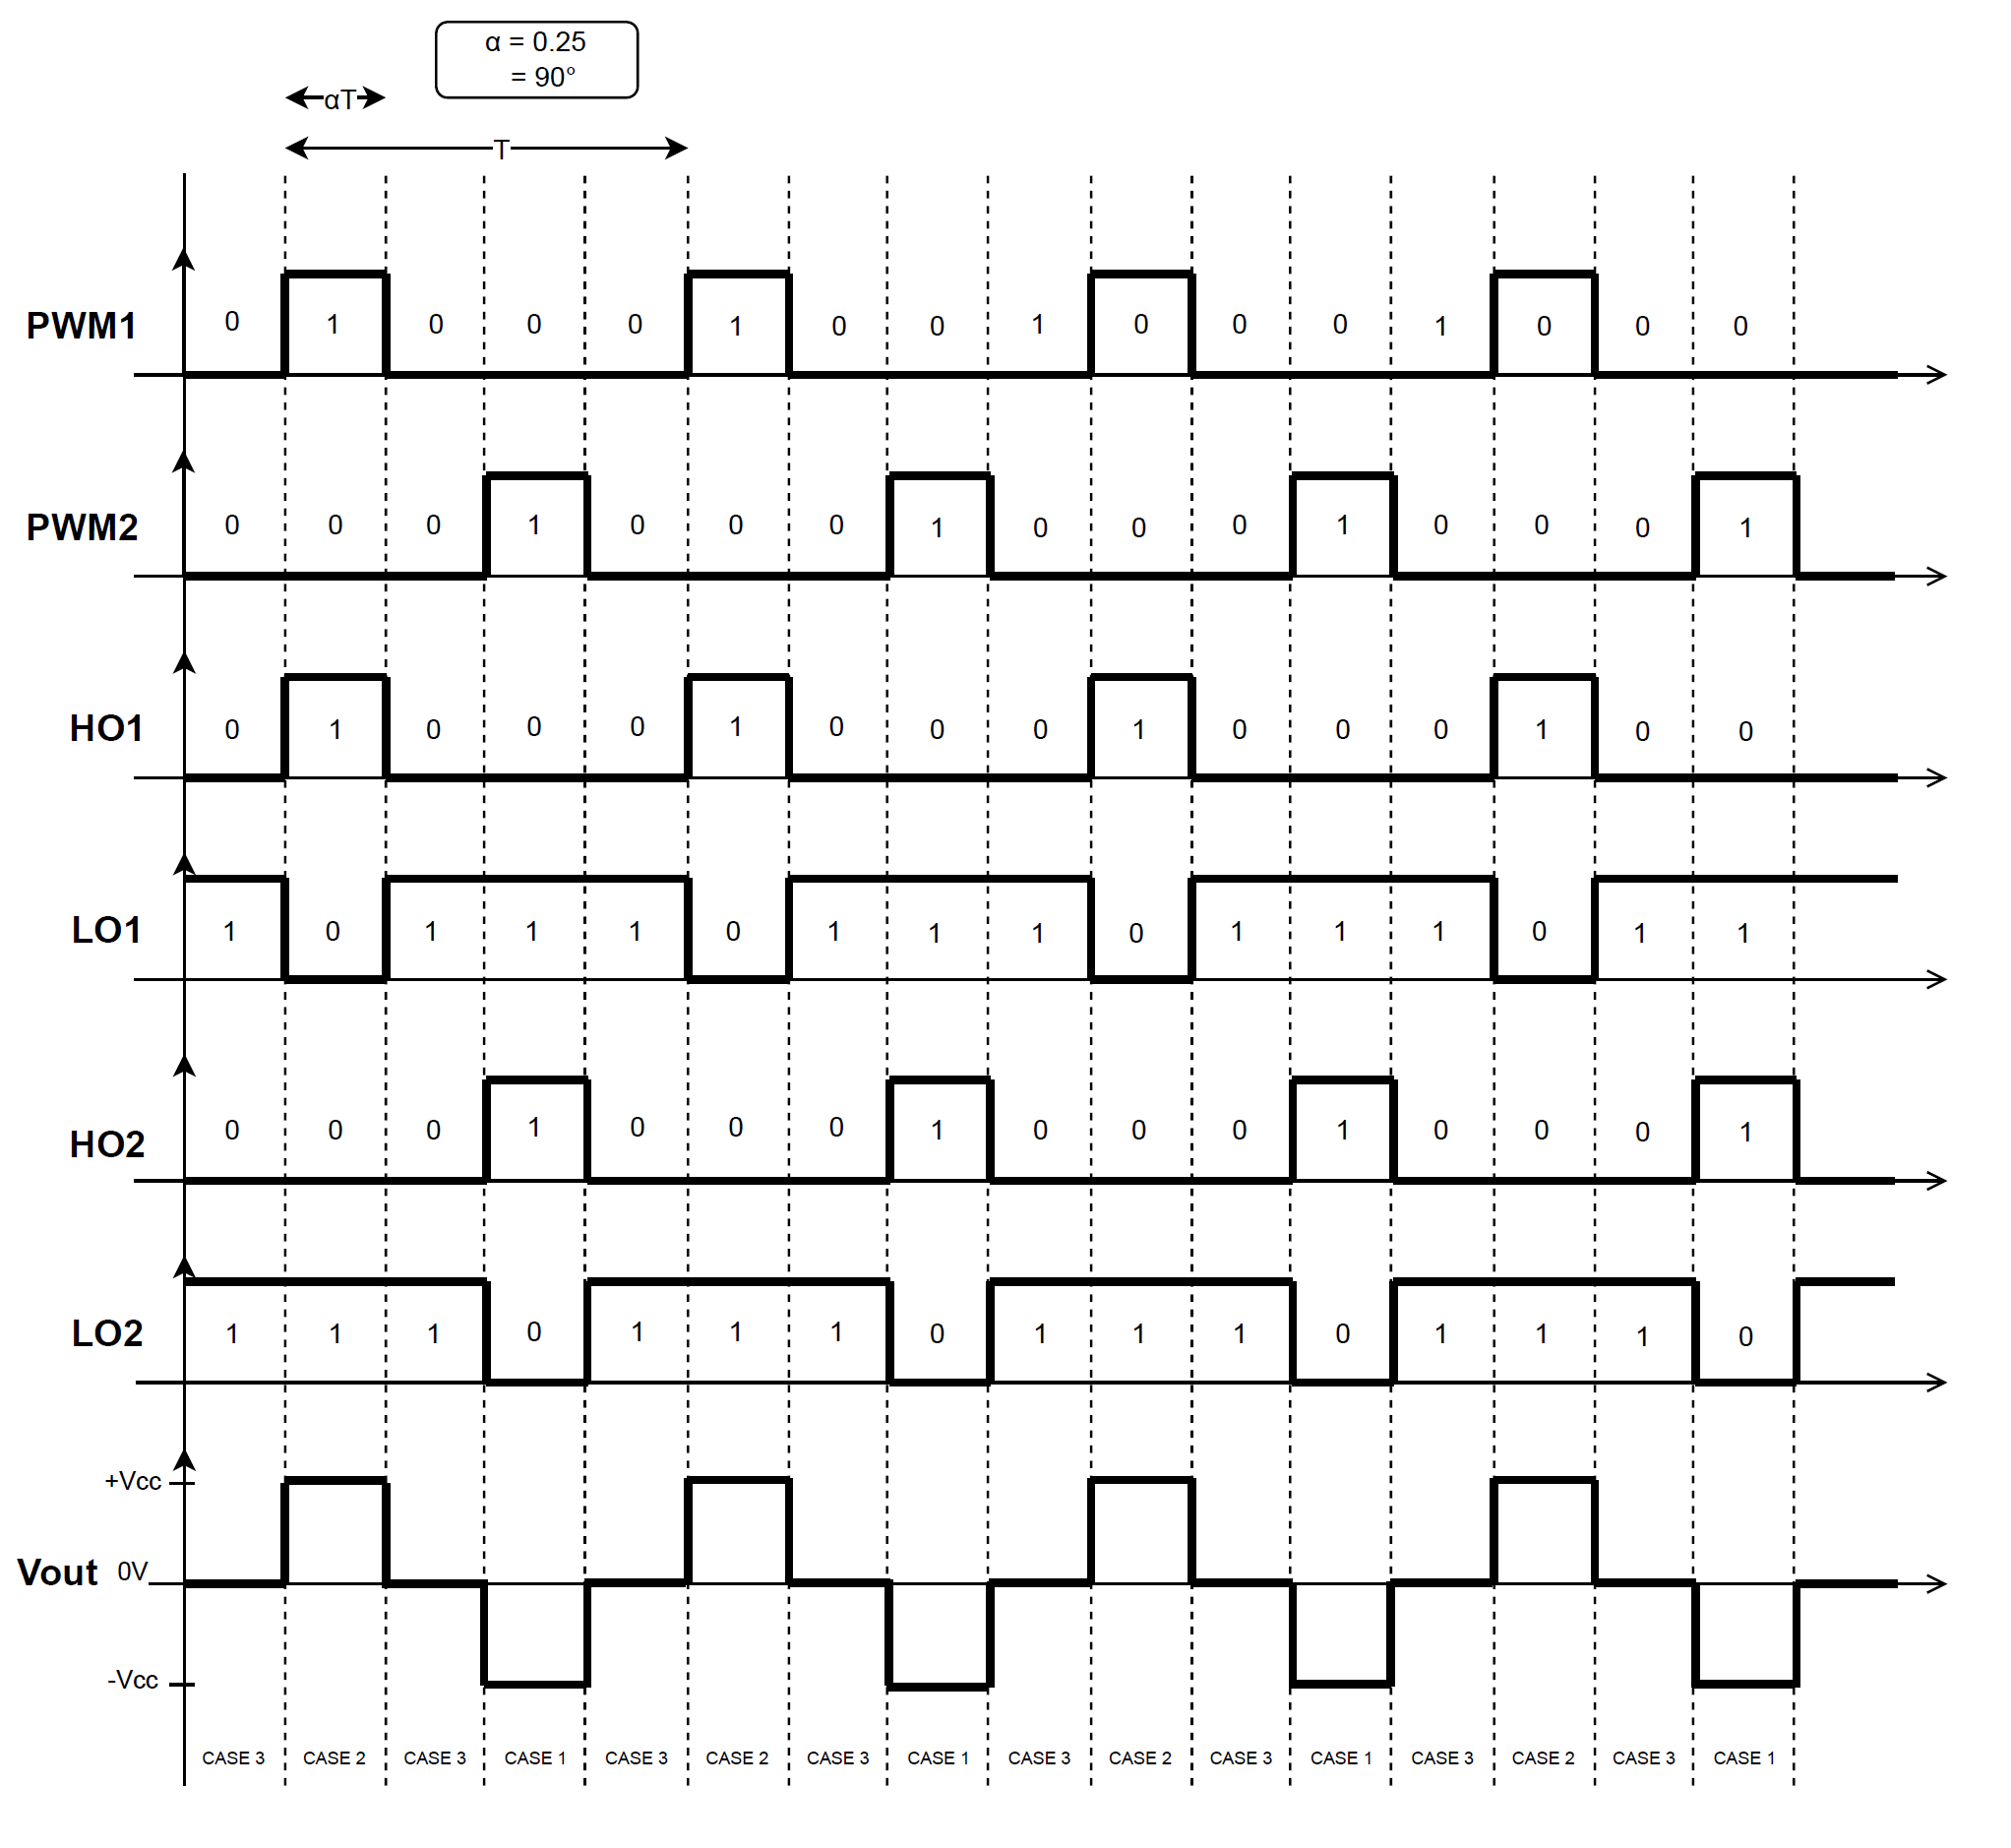
\includegraphics[width=\linewidth]{images/2.png}}
	\caption{25\% duty cycle control chronogram example}
	\label{fig}
\end{figure}

The duty cycle \(\beta\) that also must be included in the interval \([0\% ; 50\%[\) and
corresponds to the percentage of the period where the pair of MOSFET transistors (on
secondary side) [Q5, Q8] are conducting and in addition, the pair [Q6, Q7] are off.
On each side, the duty cycle must always stay under 50\% to avoid short-circuiting the
supply voltage with the ground. If the duty cycle exceeds 50\%, the two pairs of transistors
will at some point start to conduct simultaneously and therefore will damage the power
supply

\begin{figure}[htbp]
	\centering
	\begin{tabular}{|c|c|}
		\hline
		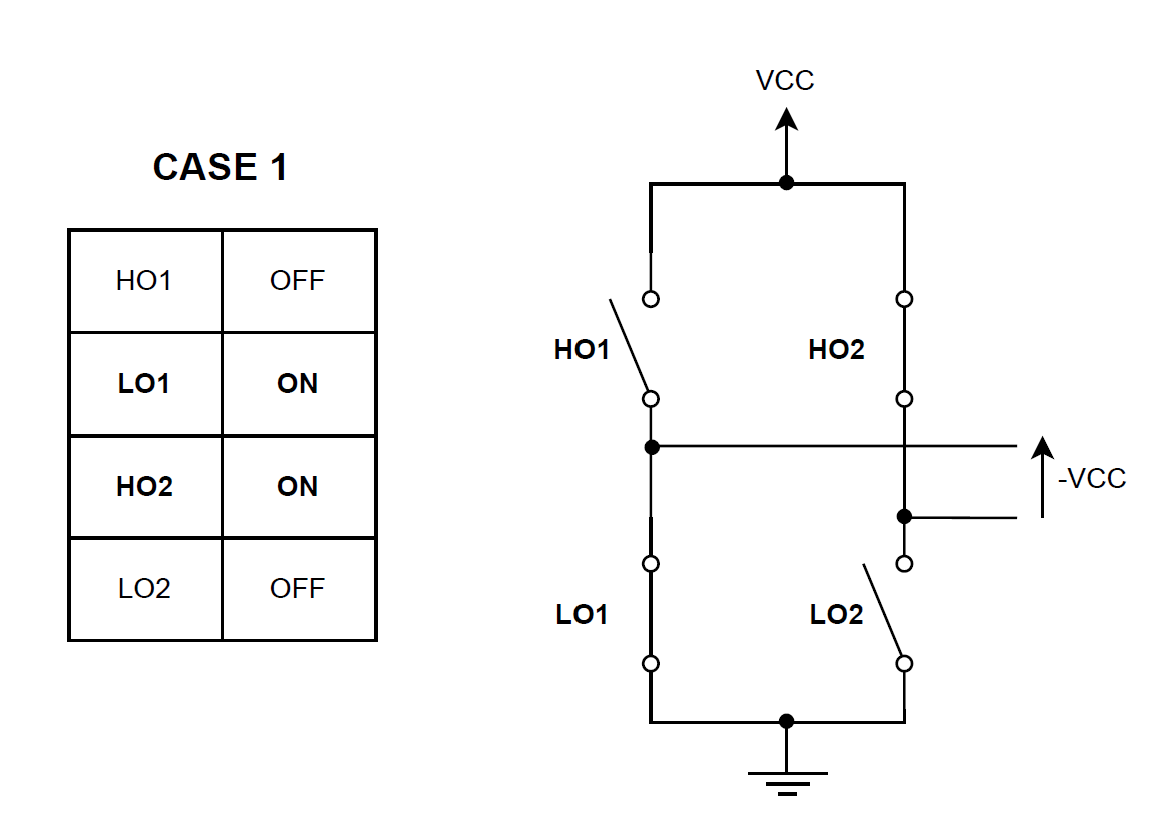
\includegraphics[width=30mm]{images/3.png} &
		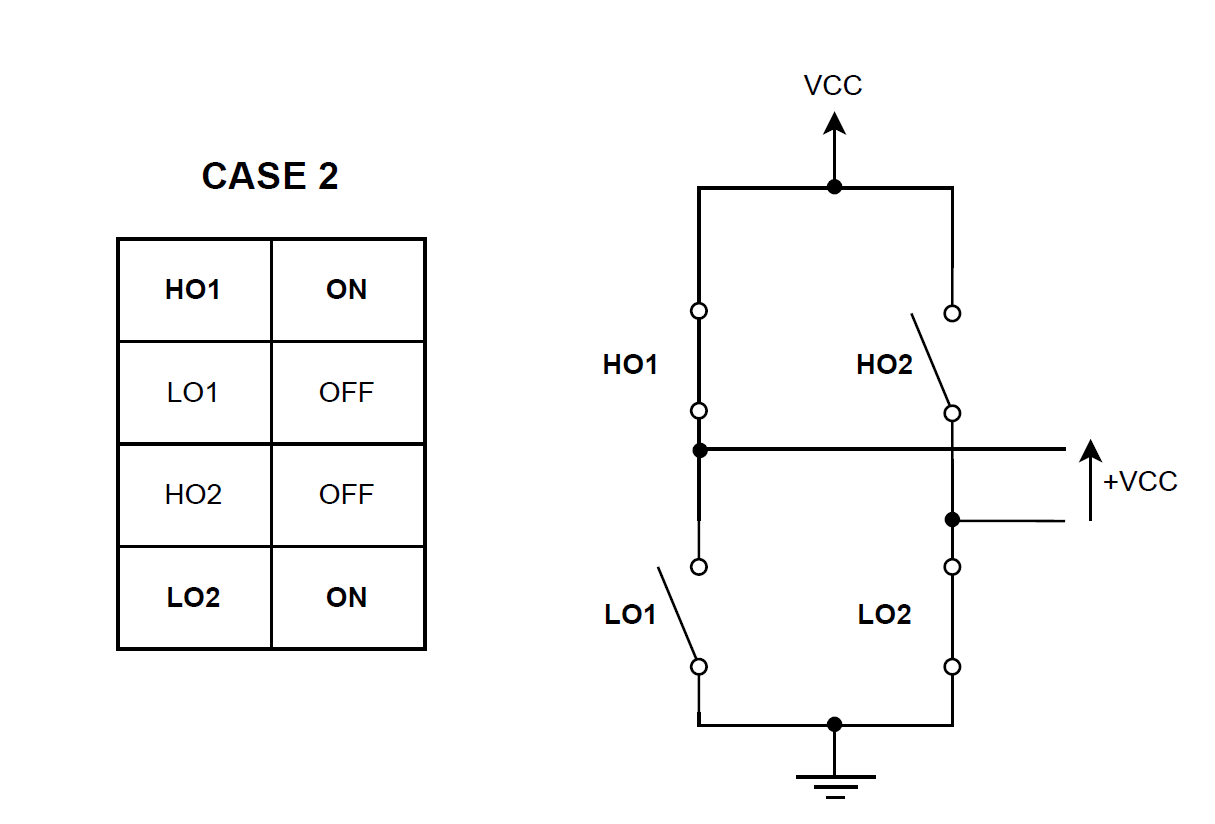
\includegraphics[width=30mm]{images/4.png} \\
		\hline
		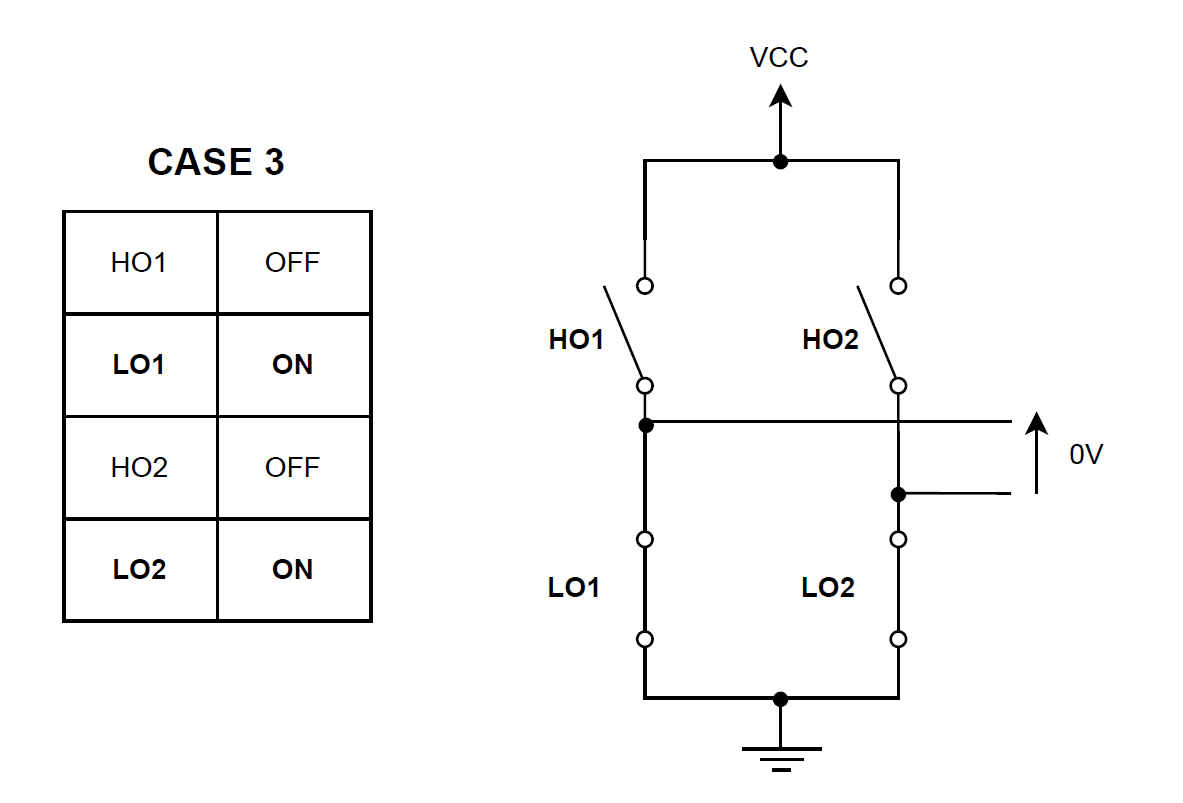
\includegraphics[width=30mm]{images/5.png} &
		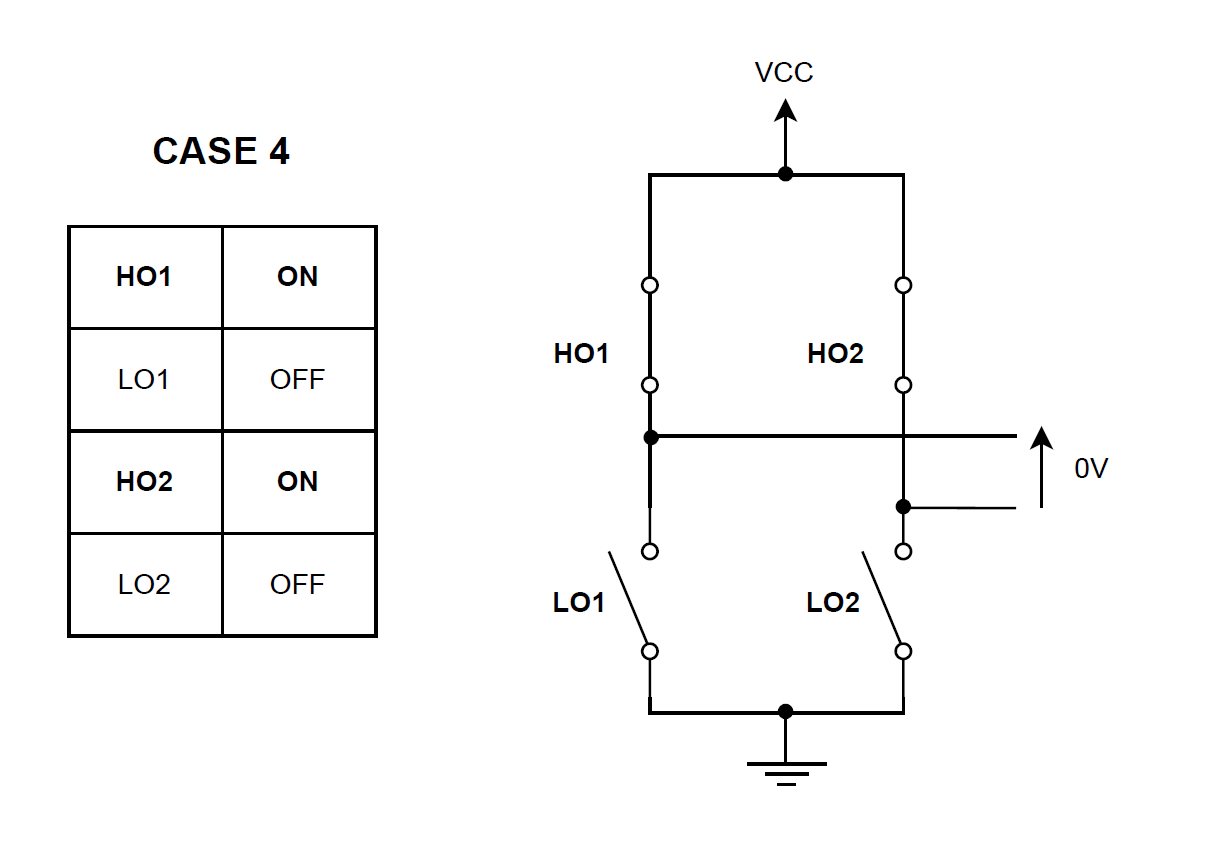
\includegraphics[width=30mm]{images/6.png} \\
		\hline
	\end{tabular}
	\caption{All differents scenarios of control}
	\label{fig}
\end{figure}

The two others parameters linked and deduce from the two duty cycle are \(\varphi_P\) and,  \(\varphi_S\)
corresponding to the phase-shift between the two legs of the converter through \(\alpha = 180^\circ - \varphi_P\) and \(\beta = 180^\circ - \varphi_S\). Since the bridge consists of two H-bridges on one side
at primary and then secondary level, there are similar dimensions on each side of the
converter.
We can express \(\alpha\) or \(\beta\) in an angle unit or with a percentage. The duty cycle is between
0 and 100\%, if we consider a period \(T\) , the time during the high state can be expressed
as \(\alpha T\) which can be called \(\tau\). So \(\tau = \alpha T\). In fact, we can express \(T\) or \(\tau\) with a time unit
\( \left(s\right) \) or with an angle unit \( (^{\circ}) \). This leads to expressing \( \alpha \) in degrees, considering a period as \( 360^{\circ} \) or linearly. Such as \(\alpha \left[^{\circ}\right] = \alpha \left[linear\right] \times 360\).

\subsection{Equations}
We based our research on the bidirectional Wireless Power Transfer System with a
series-series compensation from [1]. During the first part of our research, the circuit and
the equation associated with was analysed to have a better understanding of the circuit
and to ensure that there is no error in the paper.
For the analysis, a diagram was made to see how the H bridge works to understand how
it can be link to the simplified model of the article [1]. From the Vout chronogram, it can be
deduced that the bridge behaviour can be assimilated to a sinusoidal signal by
simplifying the bridge command with a first order approximation. From that analysis, the
simplified model was used to find a State Space Model of this circuit by considering the
transistor command as a sinusoid depending on the phase between the transistors. The
aim here is to find a usable state space model to be able to control it with a command
law.
From the simplified model, the chosen states are  \(i_p, u_cp, i_s, u_{cs}\).
To ensure that the model is usable and reliable, we have to verify the model via MATLAB
and Simulink simulation and compare the circuit simulation to our model.

\subsection{Python simulation}
In order to graphically visualize the relationship between all the mathematical relations
presented so far, a Python script was programmed. By adding a solver system linking the
functions (X), (X) and (X), and with the MatPlotLib graphics library, the plot of power
output as a function of variations in M and BETA was generated. The graphical figure
resulting from the Python simulation is shown below:
\begin{figure}[htbp]
	\centerline{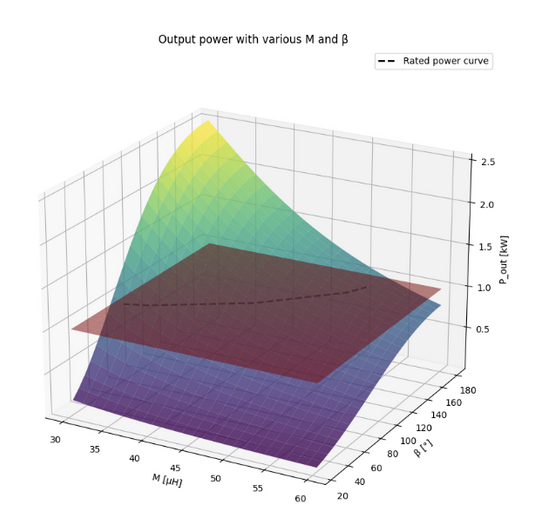
\includegraphics[width=\linewidth]{images/7.png}}
	\caption{Output power with various \(M\) and \(\beta\)}
	\label{fig}
\end{figure}
It may be worth pointing out that the article [X] contains some internal errors, notably on
the annotation of their simulation allowing the graphical representation of power output
with respect to the parameters \(M\) and \(\beta\). Indeed, for a given output power of 1 kW and
a mutual inductance \(M\) of 35 uH, the \(\beta\) angle obtained is 80.39° and not 83° as
specified in the article.

\subsection{Python simulation}
\subsubsection{LTSpice}
An LTSpice simulation was made to model the expected behaviour of the system reliably,
so that we could validate it and begin calculations to obtain its state space.
So, by selecting MOSFET power transistors commonly used in Dual Active Bridge
devices, with good efficiency to limit switching losses, and adding all the PWM control
signals (PWM 1 to 8), it is possible to obtain a complete simulation of the system. In our
case, the transistors are considered ideal, and the control output obtained corresponds
to the expectations in ideal condition. The result can be seen in the chronogram below :
\begin{figure}[htbp]
	\centerline{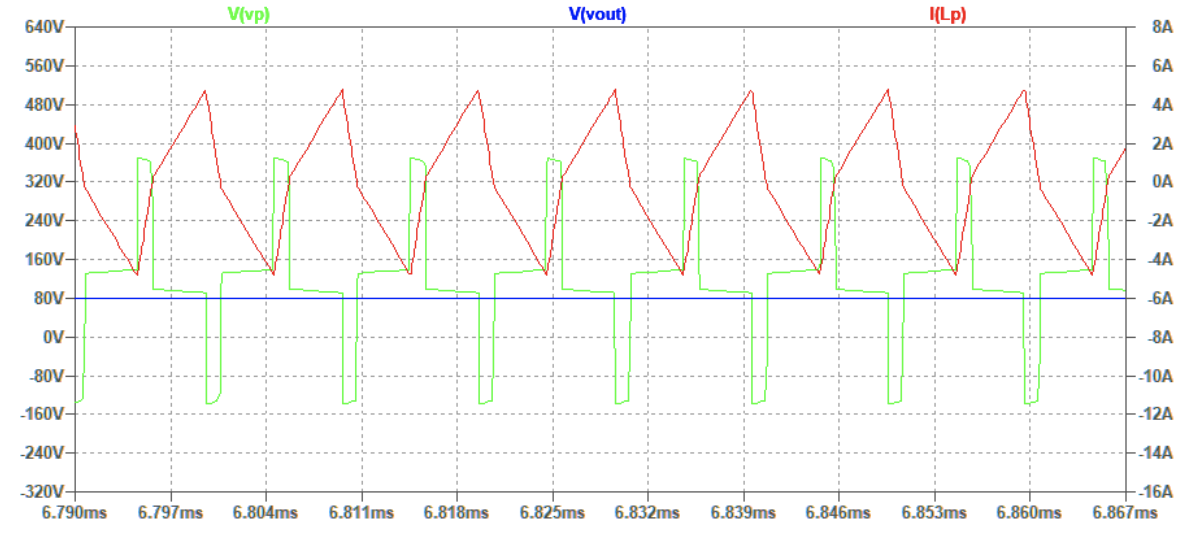
\includegraphics[width=\linewidth]{images/8.png}}
	\caption{Chronogram of output voltage \(V_P\), continus \(V_{out}\) voltage and primary current}
	\label{fig}
\end{figure}
However, in order to get closer result compared to physical reality, parasitic capacitors
in parallel of the MOSFETs was used to modelized the imperfection of the transistor. In
this case, the voltage difference across the control plates is greater.
\begin{figure}[htbp]
	\centerline{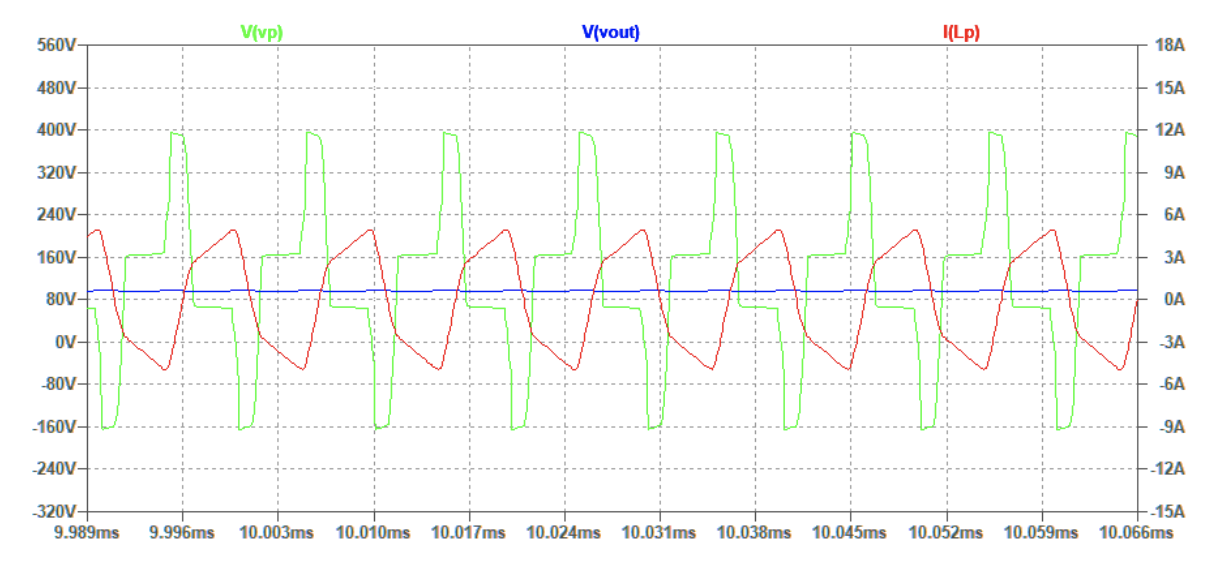
\includegraphics[width=\linewidth]{images/9.png}}
	\caption{Chronogram of output voltage \(V_P\), continus \(V_{out}\) voltage and primary current}
	\label{fig}
\end{figure}
\subsubsection{MATLAB/Simulink, electrical simulation}
As part of this study, a MATLAB/Simulink simulation has been developed in order to
validate the DAB. The main goal of this was to compare the converter behaviour obtained
from the linearized state space model with the full electric model implemented in
Simulink. This approach allows evaluating the precision and relevance of theoretical
equations, especially in terms of dynamics and response at steady state. It is a more
representative model of physical reality, integrating non-linearities and losses.
\begin{figure}[htbp]
	\centerline{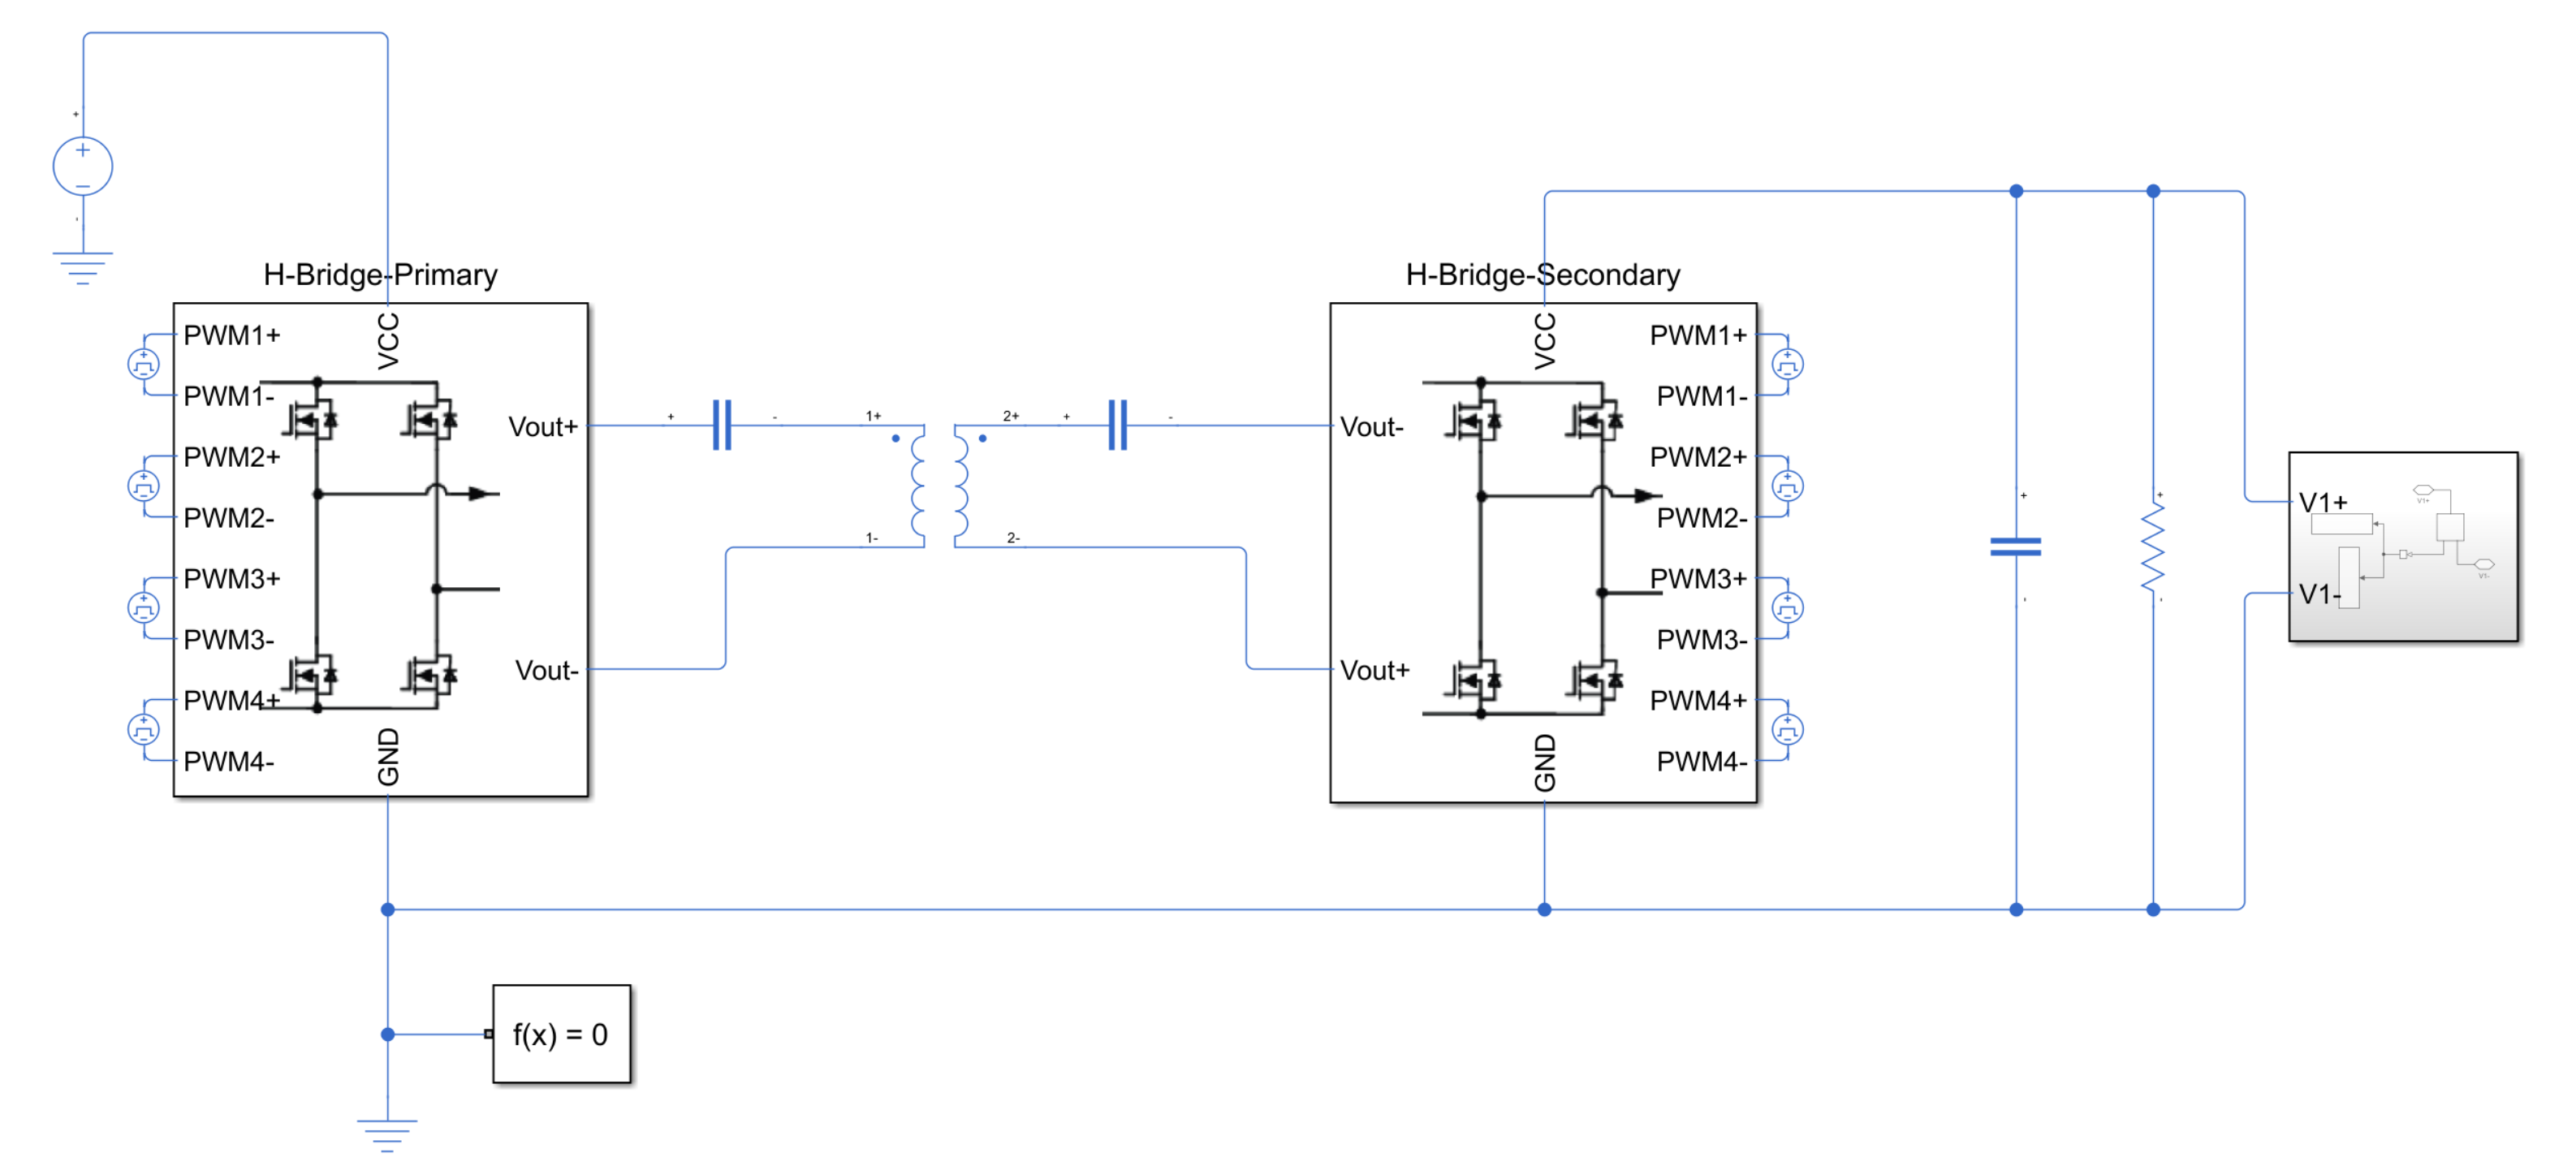
\includegraphics[width=\linewidth]{images/10.png}}
	\caption{Global schematic of the DAB into Simulink}
	\label{fig}
\end{figure}
\begin{figure}[htbp]
	\centerline{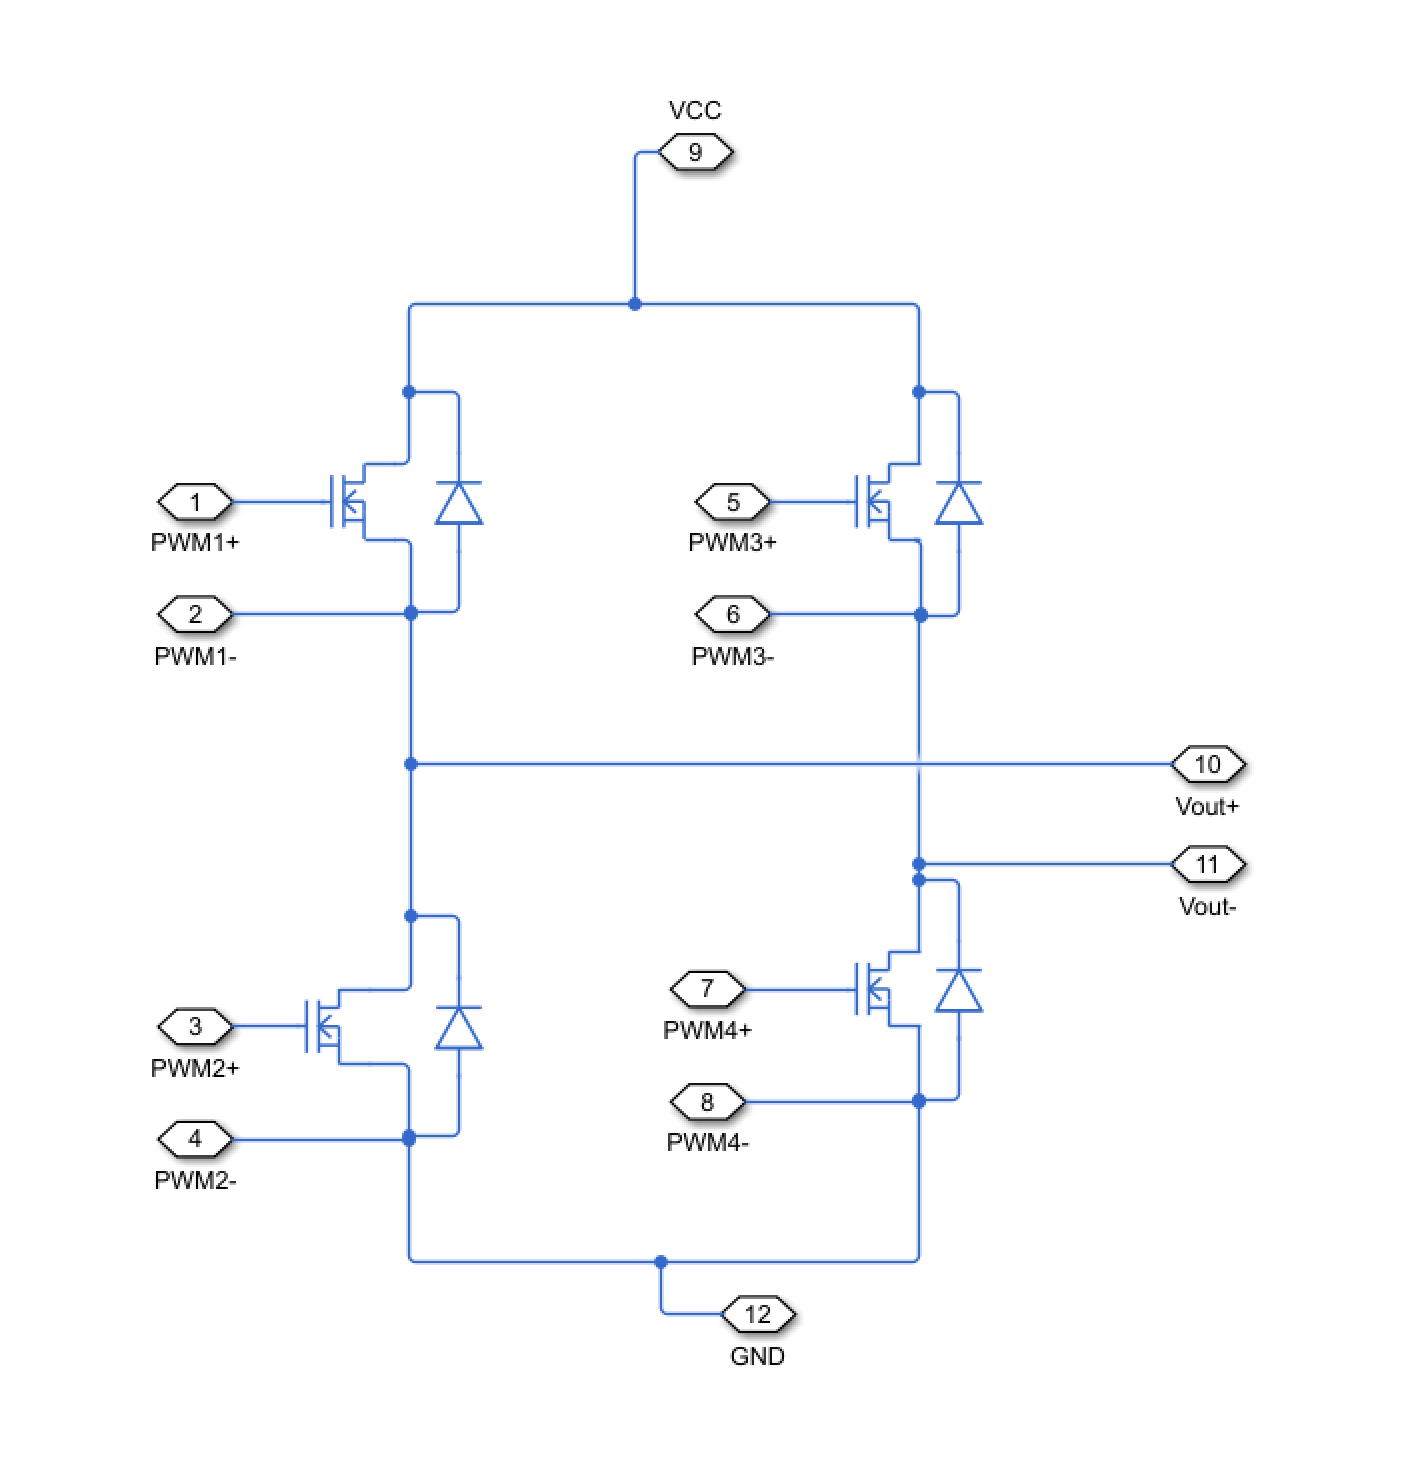
\includegraphics[height=0.25\textheight]{images/11.png}}
	\caption{Inside the H-bridge box}
	\label{fig}
\end{figure}
We tried to compare the two models through several simulations by varying the
working conditions (supply voltage, frequency, duty cycle...), with the aim of identifying
possible gap and validate the mathematical model.
\begin{figure}[htbp]
	\centerline{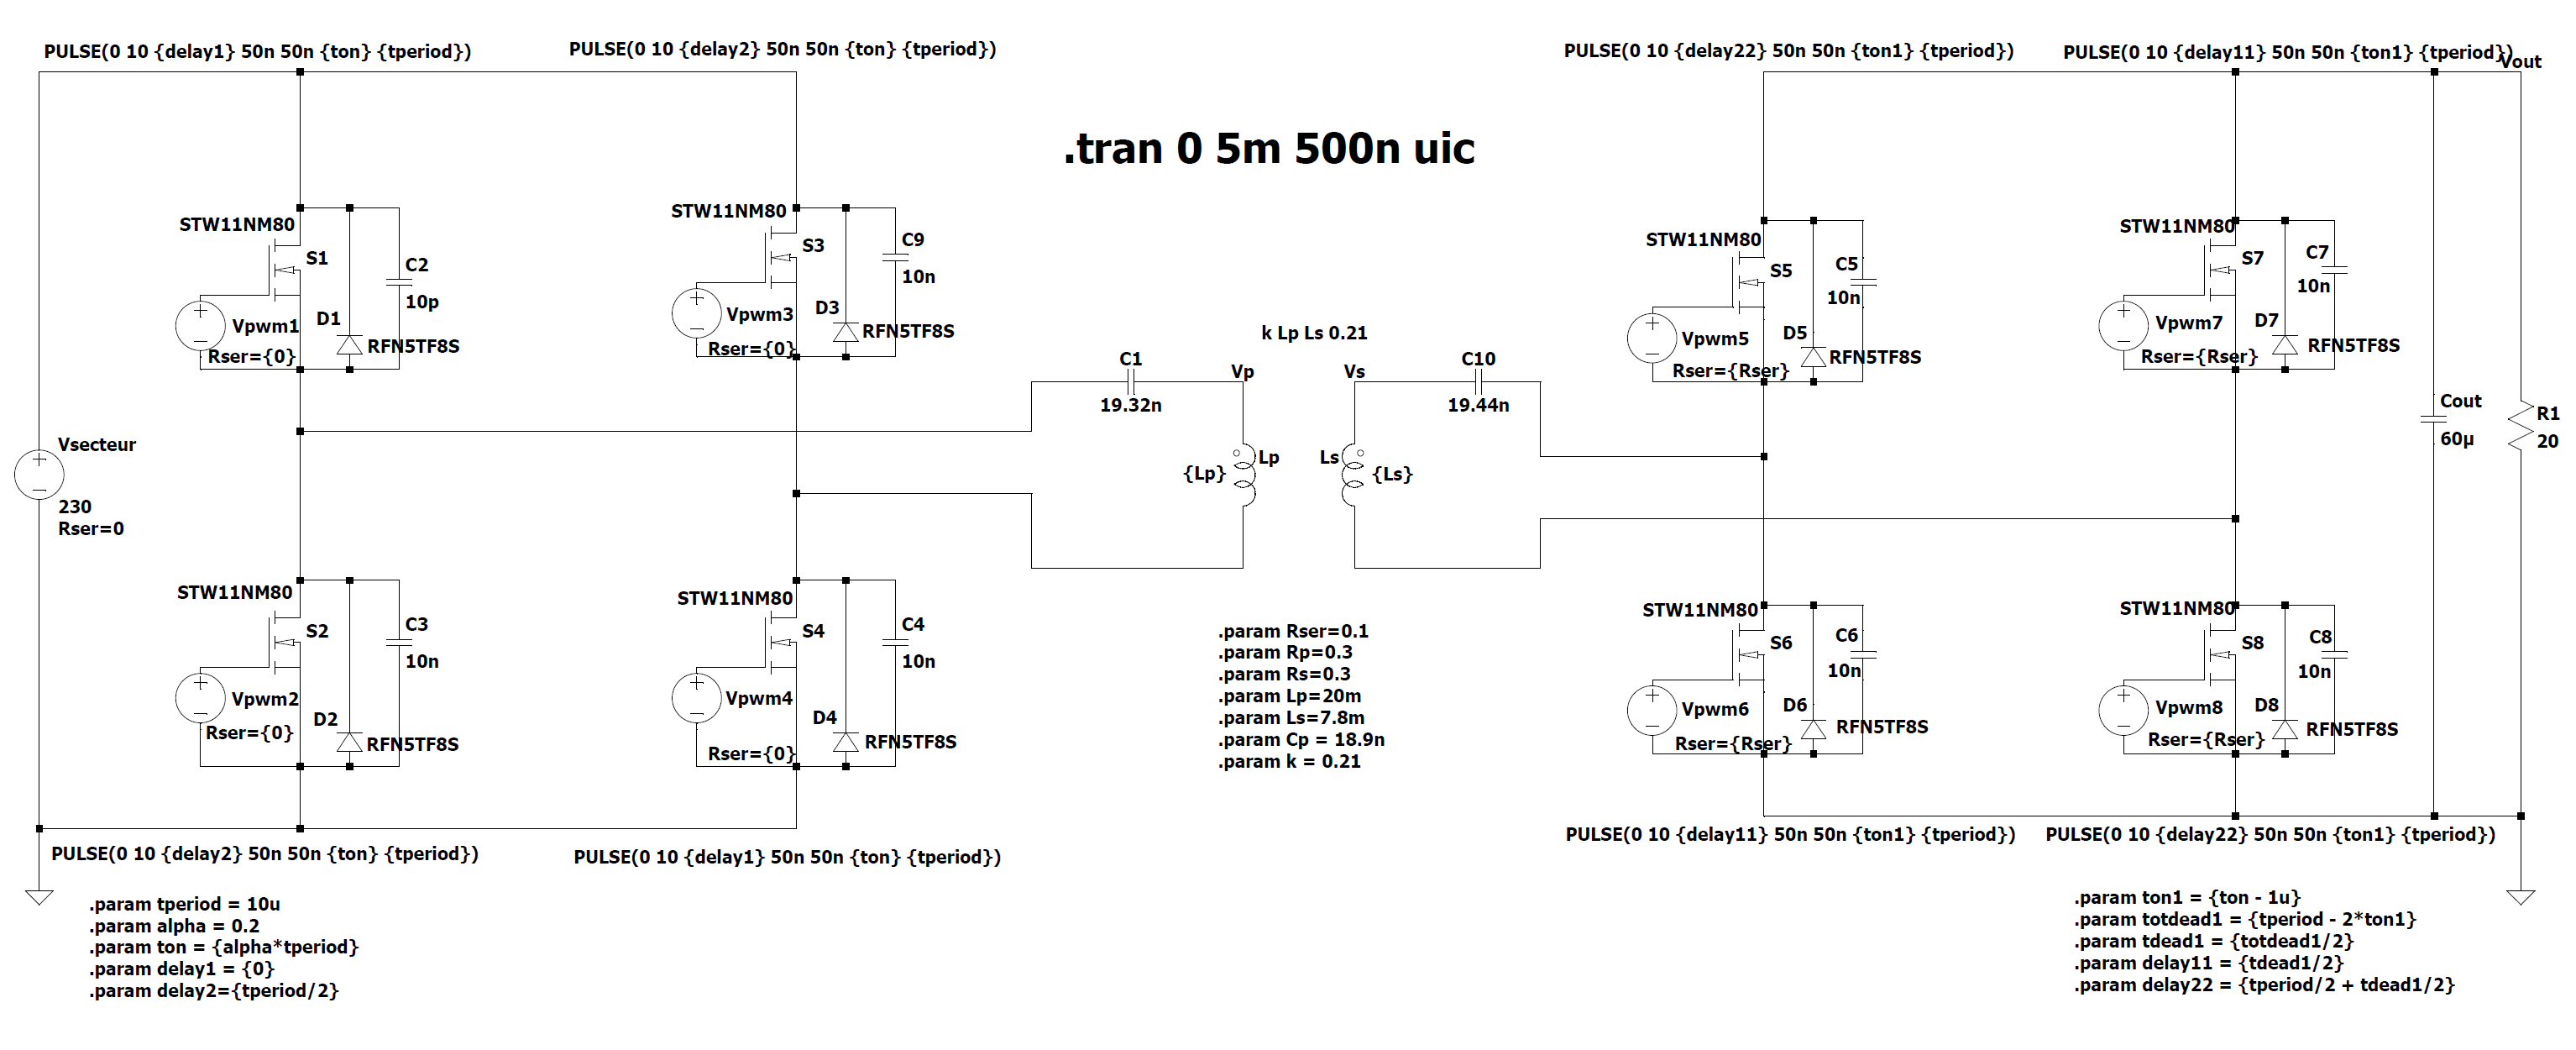
\includegraphics[width=\linewidth]{images/12.png}}
	\caption{Global schematics of the DAB into LTSpice}
	\label{fig}
\end{figure}
The LTSpice simulation was used as a reference point for the analysis of the converter
behaviour. The two models, LTSpice and Simulink, were configured with the same
component values (capacitances, inductances, parasitic resistors, etc.), as well as an
identical control of the switches (MOSFET transistors). However, despite this
consistency in terms of hardware parameters and control strategy, the behaviour
observed in the two environments differs significantly, especially regarding energy
transfer between the primary and secondary.

In the Simulink model, the logical switch control works correctly, the control signals
are applied according to the sequences planned for a DAB, but the current is not
transmitted as expected to the secondary, contrary to what is observed in the LTSpice
simulation. This divergence remains unexplained at this stage of the study, and several
tracks are considered, such as possible differences in component models, taking into
account losses or the treatment of magnetic coupling in each of the software.
An additional difficulty is that, given the complexity of the wireless resonant energy
transfer principle, we do not have a clear reference for the expected waveforms of the
output currents and voltages. This lack of reference data makes it difficult to qualitatively
analyze the simulation results and validate system behavior in Simulink.

Thus, although the control seems functional and the state space model offers an
interesting basis for analysis, the difference in behavior observed between LTSpice and
Simulink, despite the use of the same parameters, remains a critical point of our work,
requiring further investigation.

\subsubsection{State space, automatic simulation}
Measurement and Characterization of Mutual Inductance in a Coupled Coil System.

\subsection{Measurement and characterisation of mutual inductance an inductive coupling system}
\subsubsection{Reminder on series resonance}
Resonance occurs when the coil and capacitor cancel each other out. It is at this
point that the total impedance is the smallest, the lowest. The resonant frequency can
be expressed as
$$ \frac{1}{2\pi\sqrt{LC}}$$
Where \(L\) is the coil inductance (in Henry) and \(C\) is the capacitor capacitance (in Farad).
Figure XX shows a basic circuit used to visualise the resonance phenomenon, which
illustrates the typical frequency response showing a resonance peak. In Figure XX, the
measured resonance frequency is \(f_{resonant} = 159 Hz\).

\begin{figure}[htbp]
	\centerline{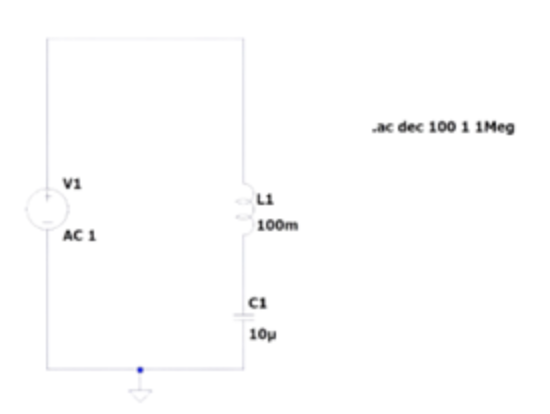
\includegraphics[width=\linewidth]{images/22.png}}
	\caption{Electronic circuit \(LC\)}
	\label{fig}
\end{figure}
\begin{figure}[htbp]
	\centerline{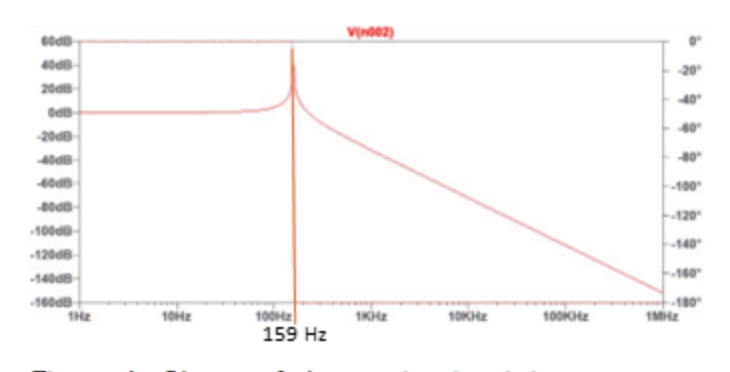
\includegraphics[width=\linewidth]{images/23.png}}
	\caption{Shape of electronic circuit in resonance}
	\label{fig}
\end{figure}

\subsubsection{Energy transfer system in near field}
The mutual inductance M was determined using different methods, where the
effect of coil misalignment was also observed. \\
\begin{itemize}
	\item Measurement of M using an oscilloscope
\end{itemize}
	A sinusoidal signal was generated using a low-frequency generator with a frequency of
100 kHz. This signal is applied to the primary side of the transmitting coil, so that the
mutual inductance M can be calculated from the circuit represented in figure XX.

\begin{figure}[htbp]
	\centerline{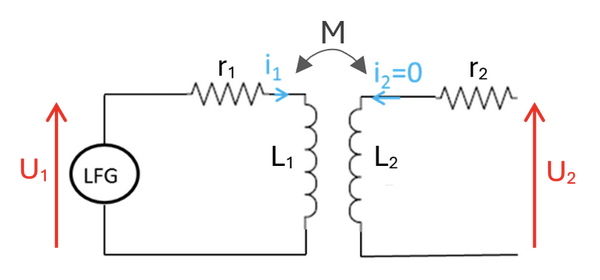
\includegraphics[width=\linewidth]{images/24.png}}
	\caption{Schematic of inductive coupling between two coils}
	\label{fig}
\end{figure}
By using as a hypothesis \(r_1 << L_1\), we can write M as
$$ M = \frac{|U_2|}{|U_1|} \times L_1 $$
where \(U_1\) is the input voltage \(V\), \(U_2\) is the output voltage \(V\) and \(L_1\) the self-inductance
\(H\).
From the input and output voltages value measured, with the oscilloscope we can
calculate the self-inductance such as
$$ M = \frac{|0.117|}{|0.362|} \times 28.3 \times 10^{-6} $$

\begin{itemize}
	\item Measurement of M using a Vectorial Network Analyzer (VNA)
\end{itemize}
We also used the VNA because, it allowed us to measure the parameters of the
scattering parameters in order to deduce the mutual inductance, and visualise the shape of these parameters in software, so that the resonance peak can be measured accurately
and directly measure the system's self-inductance.
The figure XX shows the primary, secondary inductance and other data such as the
quality factor in the VNA software.
\begin{figure}[htbp]
	\centerline{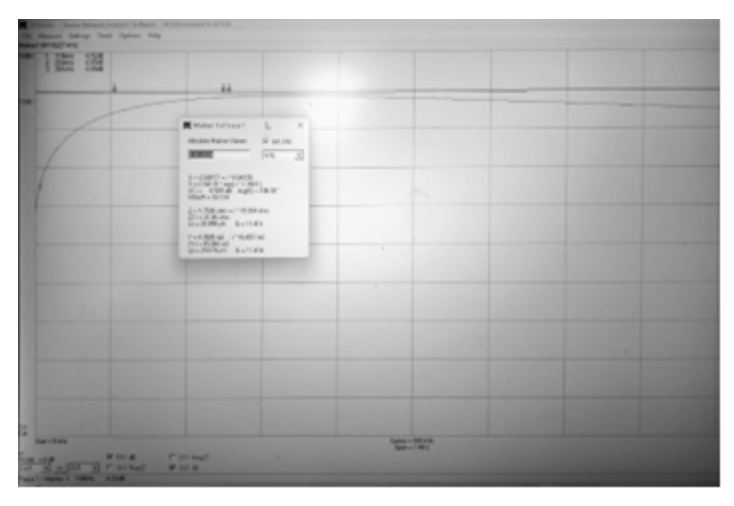
\includegraphics[width=\linewidth]{images/25.png}}
	\caption{Software interface for measuring the scattering parameters}
	\label{fig}
\end{figure}
Using the VNA, it is possible to characterize a quadripole (Figure XX). Based on the
scattering parameters (also called S-parameters) : \(S_{11}, S_{12}, S_{21}, S_{22}\), the value of the
mutual inductance can be determined.
\begin{figure}[htbp]
	\centerline{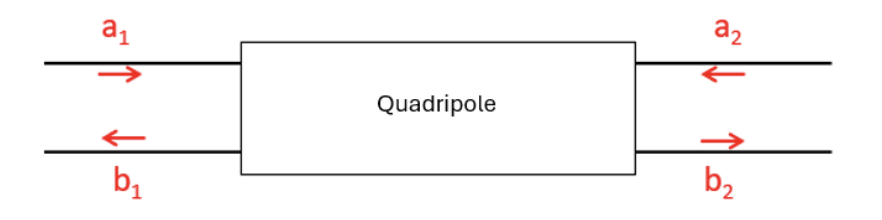
\includegraphics[width=\linewidth]{images/26.png}}
	\caption{Software interface for measuring the scattering parameters}
	\label{fig}
\end{figure}

\(S_{11} = \frac{b_1}{a_1}\) is the input port \(a_1\) reflection coefficient. \\

\(S_{12} = \frac{b_1}{a_2}\) is the reverse gain. It represents to the fraction of the signal transmitted from
port 2 to port 1. \\

\(S_{21} = \frac{b_2}{a_1}\) is the forward gain. It represents to the fraction of the signal transmitted from
port 1 to port 2. \\

\(S_{22} = \frac{b_2}{a_2}\) is the output port \(b_2\) reflection coefficient \\

These parameters are used to calculate the mutual inductance M. The measured values
obtained are
\[
S_{11} = -0.4084794 + i \times 0.3885981
\]
\[
S_{12} = -0.0878653 + i \times 0.1240676
\]
\[
S_{21} = -0.0874657 + i \times 0.1235057
\]
\[
S_{22} = +0.7230404 + i \times 0.6052605
\]
In order to compute M :
\begin{itemize}
	\item Scattering parameters must be converted to Z parameters, the matrix
	of impedance.
	\item Take the imaginary part of \(Z_{21}\)
	\item Compute M : \(\frac{Im(Z_{21}}{2\pi \times f})\)
\end{itemize}
At the end of the calculations, the value obtained for M is :
$$ |M| = 10.930 \times 10^{-6} H $$
The value of \(L_1\) and \(L_2\) were also determined via the interface
$ L_1 = 29.076 \times 10^{-6} H$ \\
$ L_2 = 28.855 \times 10^{-6} H$





\subsection{Authors and Affiliations}


\section*{Acknowledgment}

The preferred spelling of the word ``acknowledgment'' in America is without 
an ``e'' after the ``g''. Avoid the stilted expression ``one of us (R. B. 
G.) thanks $\ldots$''. Instead, try ``R. B. G. thanks$\ldots$''. Put sponsor 
acknowledgments in the unnumbered footnote on the first page.

\section*{References}

Please number citations consecutively within brackets \cite{b1}. The 
sentence punctuation follows the bracket \cite{b2}. Refer simply to the reference 
number, as in \cite{b3}---do not use ``Ref. \cite{b3}'' or ``reference \cite{b3}'' except at 
the beginning of a sentence: ``Reference \cite{b3} was the first $\ldots$''

Number footnotes separately in superscripts. Place the actual footnote at 
the bottom of the column in which it was cited. Do not put footnotes in the 
abstract or reference list. Use letters for table footnotes.

Unless there are six authors or more give all authors' names; do not use 
``et al.''. Papers that have not been published, even if they have been 
submitted for publication, should be cited as ``unpublished'' \cite{b4}. Papers 
that have been accepted for publication should be cited as ``in press'' \cite{b5}. 
Capitalize only the first word in a paper title, except for proper nouns and 
element symbols.

For papers published in translation journals, please give the English 
citation first, followed by the original foreign-language citation \cite{b6}.

\begin{thebibliography}{00}
\bibitem{b1} G. Eason, B. Noble, and I. N. Sneddon, ``On certain integrals of Lipschitz-Hankel type involving products of Bessel functions,'' Phil. Trans. Roy. Soc. London, vol. A247, pp. 529--551, April 1955.
\bibitem{b2} J. Clerk Maxwell, A Treatise on Electricity and Magnetism, 3rd ed., vol. 2. Oxford: Clarendon, 1892, pp.68--73.
\bibitem{b3} I. S. Jacobs and C. P. Bean, ``Fine particles, thin films and exchange anisotropy,'' in Magnetism, vol. III, G. T. Rado and H. Suhl, Eds. New York: Academic, 1963, pp. 271--350.
\bibitem{b4} K. Elissa, ``Title of paper if known,'' unpublished.
\bibitem{b5} R. Nicole, ``Title of paper with only first word capitalized,'' J. Name Stand. Abbrev., in press.
\bibitem{b6} Y. Yorozu, M. Hirano, K. Oka, and Y. Tagawa, ``Electron spectroscopy studies on magneto-optical media and plastic substrate interface,'' IEEE Transl. J. Magn. Japan, vol. 2, pp. 740--741, August 1987 [Digests 9th Annual Conf. Magnetics Japan, p. 301, 1982].
\bibitem{b7} M. Young, The Technical Writer's Handbook. Mill Valley, CA: University Science, 1989.
\end{thebibliography}

\end{document}
